\chapter{K vecinos más próximos}\label{Chapter5} 
% chktex-file 8
% chktex-file 12
% chktex-file 13
% chktex-file 44

En teoría, siempre se desearía predecir respuestas cualitativas usando el clasificador de Bayes. Pero para datos reales, no se conoce la distribución condicional de $Y$ dado $X$, por lo que calcular el clasificador de Bayes es imposible. Por lo tanto, el clasificador de Bayes sirve como un estándar inalcanzable contra el cual comparar otros métodos. Muchos enfoques intentan estimar la distribución condicional de $Y$ dado $X$, y luego clasificar una observación dada a la clase con la mayor probabilidad estimada. Uno de estos métodos es el clasificador de $K$-vecinos más próximos (KNN). 

\section{Algoritmo KNN}

Sea un entero positivo $K$ y una observación de prueba $x_0$, el clasificador KNN primero identifica los $K$ puntos en los datos de entrenamiento que están más cerca de $x_0$, representados por $\mathcal{N}_0$ (generalmente se usa la distancia euclidiana). Luego estima la probabilidad condicional para la clase $j$ como la fracción de puntos en $\mathcal{N}_0$ cuyos valores de respuesta son iguales a $j$:
\begin{equation}
\Pr(Y = j | X = x_0) = \frac{1}{K} \sum_{i \in \mathcal{N}_0} I(y_i = j)
\label{eq:2.12}
\end{equation}

Finalmente, KNN aplica la regla de Bayes y clasifica la observación de prueba $x_0$ a la clase con la mayor probabilidad (los empates se resuelven de forma aleatoria). Es importante que las características de entrada estén estandarizadas (media 0 y varianza 1), pero en este método las salidas no tienen por qué estarlo. \\

\begin{figure}[h]
\centering
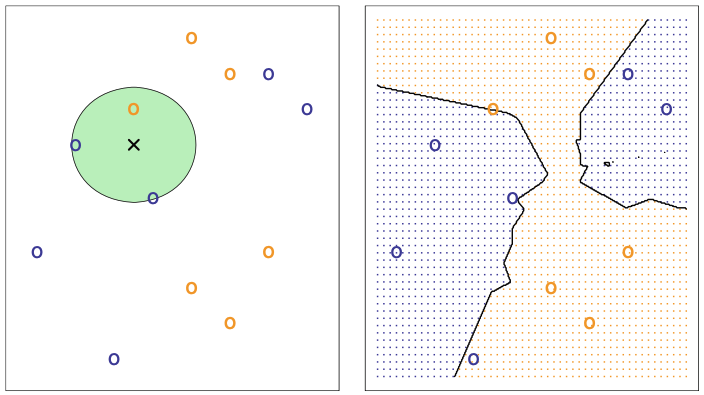
\includegraphics[width=0.5\textwidth]{fotos/10.png}
\caption{El enfoque KNN, usando $K = 3$, se ilustra en una situación simple con seis observaciones azules y seis observaciones naranjas. Izquierda: una observación de prueba para la cual se desea una etiqueta de clase predicha se muestra como una cruz negra. Se identifican los tres puntos más cercanos a la observación de prueba, y se predice que la observación de prueba pertenece a la clase que ocurre con mayor frecuencia, en este caso azul. Derecha: La frontera de decisión KNN para este ejemplo se muestra en negro. La cuadrícula azul indica la región en la cual una observación de prueba será asignada a la clase azul, y la cuadrícula naranja indica la región en la cual será asignada a la clase naranja.}
\label{fig:2.14}
\end{figure}

A pesar de que es un enfoque muy simple, KNN puede producir clasificadores que están sorprendentemente cerca del clasificador de Bayes óptimo, mostrando éxito en frontera de decisión muy irregulares. La figura \ref{fig:2.15} muestra la frontera de decisión KNN, usando $K = 7$, cuando se aplica al conjunto de datos simulado más grande de la figura \ref{fig:2.13}. Nótese que aunque el clasificador KNN no conoce la distribución verdadera, la frontera de decisión KNN está muy cerca de la del clasificador de Bayes. \\

\begin{figure}[h]
\centering
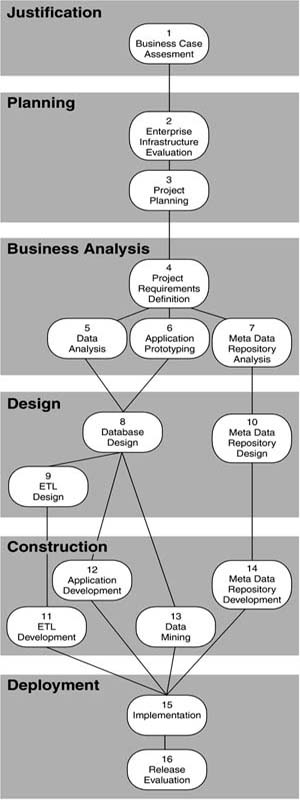
\includegraphics[width=0.6\textwidth]{fotos/11.png}
\caption{Ejemplo simulado de clasificación KNN con dos clases.}
\label{fig:2.15}
\end{figure}

\begin{figure}[h]
\centering
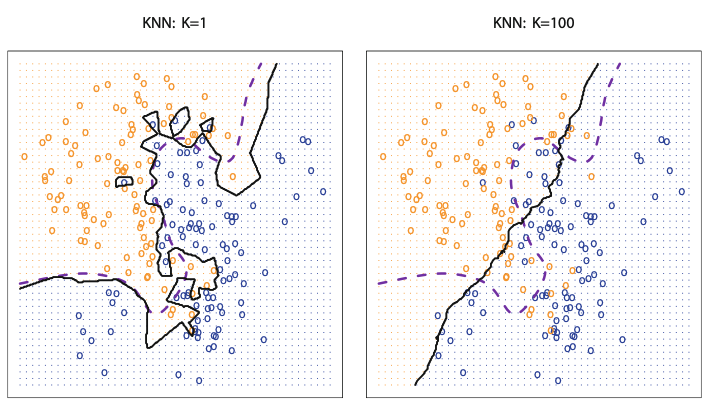
\includegraphics[width=0.6\textwidth]{fotos/12.png}
\caption{Una comparación de las fronteras de decisión KNN (curvas negras sólidas) obtenidas usando $K = 1$ y $K = 100$. La frontera de decisión de Bayes se muestra como una línea discontinua púrpura.}
\label{fig:2.16}
\end{figure}

La elección de $K$ tiene un efecto drástico en el clasificador KNN obtenido. La figura \ref{fig:2.16} muestra dos ajustes KNN a los datos simulados de la figura \ref{fig:2.13}, usando $K = 1$ y $K = 100$. Cuando $K = 1$, la frontera de decisión es excesivamente flexible y encuentra patrones en los datos que no corresponden a la frontera de decisión de Bayes. Esto corresponde a un clasificador que tiene bajo \textit{bias} pero muy alta varianza. A medida que $K$ crece, el método se vuelve menos flexible y produce una frontera de decisión que es casi lineal. Esto corresponde a un clasificador de baja varianza pero alto \textit{bias}. \\

Al igual que en el contexto de regresión, no hay una relación estrecha entre la tasa de error de entrenamiento y la tasa de error de prueba. Con $K = 1$, la tasa de error de entrenamiento de KNN es 0, pero la tasa de error de prueba puede ser bastante alta. En general, a medida que se usan métodos de clasificación más flexibles, la tasa de error de entrenamiento disminuirá pero la tasa de error de prueba puede no hacerlo. En la figura \ref{fig:2.17} se han graficado los errores de prueba y de entrenamiento de KNN como una función de $1/K$. A medida que $1/K$ aumenta, el método se vuelve más flexible. Como en el contexto de regresión, la tasa de error de entrenamiento disminuye consistentemente a medida que aumenta la flexibilidad. Sin embargo, el error de prueba exhibe una forma característica de U, disminuyendo al principio (con un mínimo en aproximadamente $K = 10$) antes de aumentar nuevamente cuando el método se vuelve excesivamente flexible y sobreajusta. \\

\begin{figure}[H]
\centering
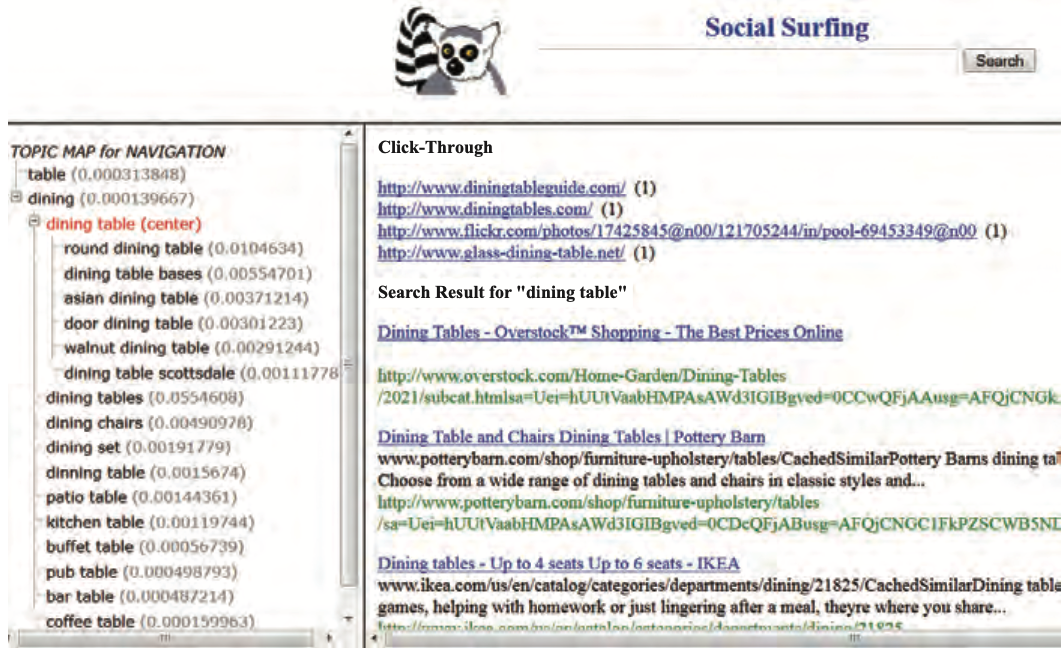
\includegraphics[width=0.4\textwidth]{fotos/13.png}
\caption{La tasa de error de entrenamiento KNN (azul, 200 observaciones) y la tasa de error de prueba (naranja, 5,000 observaciones) en los datos de la figura \ref{fig:2.13}, a medida que el nivel de flexibilidad (evaluado usando $1/K$) aumenta, o equivalentemente, a medida que el número de vecinos $K$ disminuye. La línea discontinua negra indica la tasa de error de Bayes. La irregularidad de las curvas se debe al pequeño tamaño del conjunto de datos de entrenamiento.}
\label{fig:2.17}
\end{figure}

\subsection{Alta dimensionalidad}

\begin{figure}[h]
\centering
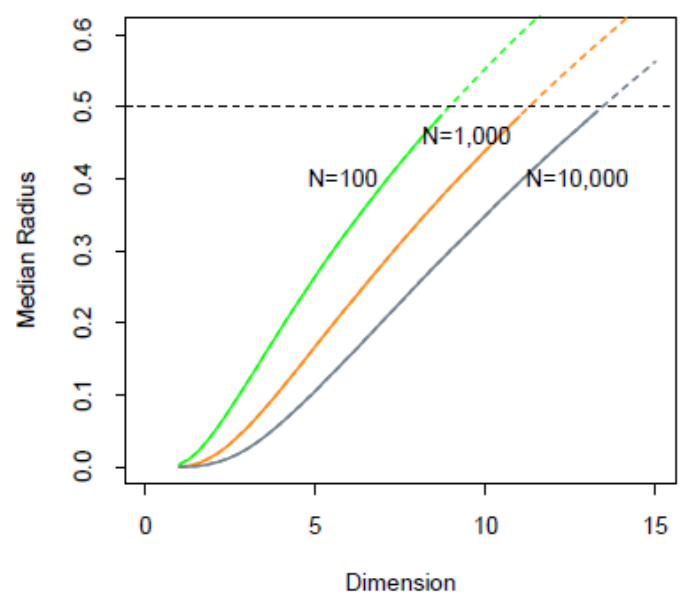
\includegraphics[width=0.45\textwidth]{fotos/20.png}
\caption{La mediana de la distancia al vecino más cercano en un hipercubo de dimensión $p$ con lados [-0.5, 0.5] en función del número de observaciones, $N$.}
\label{fig:5.18}
\end{figure}

En espacios de gran dimensionalidad, el vecino más próximo puede estar muy lejos; esto aumenta el \textit{bias} del clasificador KNN. Supongamos un hipercubo de dimensión $p$ con lados [-0.5, 0.5], la mediana del radio (o distancia) al vecino más cercano es función del número de observaciones, $N$:
\begin{equation}
\text{median}(R) = v_p^{-1/p} \left(1 - \left(\frac{1}{2}\right)^{1/N}\right)^{1/p}
\end{equation}

Si se representa esto para distintos valores de $N$, vemos que se aproxima rápidamente a la frontera del hipercubo, 0.5 (ver figura \ref{fig:5.18}). 

\subsection{Consideraciones computacionales}

La carga computacional de este algoritmo viene dada por la búsqueda de vecinos y el almacenamiento de todo el conjunto de entrenamiento. Para un conjunto de $N$ observaciones y $p$ predictores, se necesitas $N \cdot p$ operaciones para encontrar los vecinos. \\

Como soluciones, hay algoritmos más rápidos para encontrar los vecinos más próximos y se pueden almacenar los datos más importantes, cerca de la frontera de decisión y en el lado correcto de esta.


\section{Ejercicio}

\begin{example}
\textbf{Dado el siguiente conjunto de datos de clasificación con 6 observaciones, 3 variables de entrada y una variable de salida:}

\begin{table}[H]
\centering
\begin{tabular}{ccccc}
\hline \hline
Observación & $X_1$ & $X_2$ & $X_3$ & Y \\ \hline \hline
1           & 0  & 3  & 2  & 1 \\ 
2           & 3  & 0  & 3  & 0 \\ 
3           & 0  & 3  & -1 & 0 \\ 
4           & 3  & 0  & 0  & 1 \\ 
5           & 1  & 2  & 1  & 1 \\ 
6           & 2  & 1  & 0  & 0 \\ \hline
\end{tabular}
\end{table}

\textbf{Suponiendo que se quiere hace la predicción de la variable de salida para $X_i = 0, \; i = 1, 2, 3$ mediante KNN.}
\begin{enumerate}
\item \textbf{Computar la distancia entre cada observación y el punto de *test*.}
\item \textbf{¿Cuál es la predicción para $K = 1$?¿Por qué?}
\item \textbf{¿Cuál es la predicción para $K = 3$?¿Por qué?} 
\end{enumerate}

Lo primero sería calcular la distancia euclidiana de cada observación al punto de test, que en este caso es $X_i = 0, \; i = 1, 2, 3$. La distancia euclidiana entre dos puntos $A = (x_1, x_2, x_3)$ y $B = (x_1', x_2', x_3')$ es:
\begin{equation*}
d(A, B) = \sqrt{(x_1' - x_1)^2 + (x_2' - x_2)^2 + (x_3' - x_3)^2}
\end{equation*}

\begin{table}[H]
\centering
\begin{tabular}{ccccccc}
\hline 
Observación & 1 & 2 & 3 & 4 & 5 & 6 \\ \hline
Distancia al punto test & 3.6056 & 4.2426 & 3.1623 & 3 & 2.4495 & 2.2361 \\ \hline
\end{tabular}
\end{table}

Así, si se toma $K = 1$, el vecino más próximo es la observación 6, que pertenece a la clase 0. Por lo tanto, la predicción para $K = 1$ es 0. \\

Si tomamos $K = 3$, los tres vecinos más cercanos son las observaciones 4, 5 y 6, que pertenecen a las clases 1, 1 y 0 respectivamente. Por lo tanto, la predicción para $K = 3$ es 1.
\end{example}